\scanpage{52}
\uline{Biextensions \unsure{sous hyp. de|sans hyp. de} rigidité}

$A,G$ faisceaux abéliens sur topos $\unsure{S|\mathcal S}$,
\begin{center}
\begin{tabular}{@{}l@{}l@{}}
$f:A\longrightarrow S$ &
\begin{tikzpicture}[overlay,baseline=0pt,x=1em,y=1ex]
\draw (-.2,.5) .. controls (.4,-.7) and (1.3,-2.2) .. (1.8,-2.5);
\end{tikzpicture}\\
& \hspace{1.6em}objet final
\end{tabular}
\end{center}

a) Supposons $\underline{\operatorname{Hom}}_{\unsure{grs|gr|gts|gtes}}(A,G)\simeq0$. Alors
\[
\operatorname{Ext}^1(A,G)\xrightarrow{\sim}H^0(S,\underline{\operatorname{Ext}}(A,G))
\]
donc la connaissance du \uline{faisceau} $\underline{\operatorname{Ext}}(A,G)$ implique celle de $\operatorname{Ext}(A,G)$ et ts des $\operatorname{Ext}(A_{\unsure{\bar s|T|\bar S}},G_{\unsure{\bar s|T|\bar S}})$.

b) Supposons $\underline{\operatorname{Hom}}_{pct}(A,G)=0$, Alors
\margin{\begingroup
\setbox0=\hbox{i.e. $f_{\unsure{*|\alpha}}(G_A)\xleftarrow{\sim}G$}
\dimen0=\wd0 \advance\dimen0 by 8pt
\dimen2=\ht0 \advance\dimen2 by \dp0 \advance\dimen2 by 8pt
\leavevmode\rlap{\raisebox{\dimexpr-\dp0-4pt\relax}{%
\begin{tikzpicture}[x={\dimexpr\dimen0/490\relax},y={\dimexpr-\dimen2/80\relax},line width=.3pt]
\path[use as bounding box] (0,0) rectangle (490,80);
\draw (28,75) .. controls (26,67) and (38,70) .. (65,69) -- (453,68) .. controls (475,70) and (478,62) .. (476,56);
\end{tikzpicture}}}%
\kern4pt\box0\kern4pt\endgroup}
\margin{\figure{\begin{tikzpicture}\draw(0,0)--(0,-.35);\end{tikzpicture}} Hom (pas \unsure{néc\textsuperscript{t}} multiplicatifs)\\qui respectent la section\\\unsure{unités|unité}}
\begin{center}
\begin{tabular}{@{}r@{\quad}l@{}}
$H^1(A,A_G)\simeq H^1(S,G)\times$ & $\vcenter{\hbox{\begingroup
\setbox0=\hbox{$\displaystyle H^0(S,R^1f_{\unsure{*|\alpha}}(G_A)$}
\dimen0=\wd0 \advance\dimen0 by 18pt
\dimen2=\ht0 \advance\dimen2 by \dp0 \advance\dimen2 by 16pt
\rlap{\raisebox{\dimexpr-\dp0-8pt\relax}{%
\begin{tikzpicture}[x={\dimexpr\dimen0/390\relax},y={\dimexpr-\dimen2/105\relax},line width=.3pt]
\path[use as bounding box] (0,0) rectangle (390,105);
\draw (30,78) .. controls (140,83) and (300,82) .. (365,80) .. controls (375,81) and (377,78) .. (372,73);
\end{tikzpicture}}}%
\kern9pt\box0\kern9pt\endgroup}}$\\
& \hspace{1em}\rotatebox{90}{$\simeq$}\\
& Classes \unsure{à|:} isom près de $G_A$-torseurs\\
& \deleted{\unsure{fou}} rigidi\uline{\unsure{fiés|fié}} rel. à $e_A$\\
& \hspace{1em}\rotatebox{90}{$\simeq$}\\
& Classes de \deleted{torseurs} $G_A$-torseurs\\
& rigidi\uline{fiables} rel. à $e_A$.\\
\end{tabular}
\end{center}
\margin{\figure{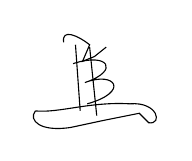
\begin{tikzpicture}[x=.03cm,y=-.03cm]
\draw (25,13) .. controls (24,7) and (31,10) .. (36,14) -- (33,21) -- (38,19) -- (43,15);
\draw (30,14) -- (32,42);
\draw (36,15) -- (39,44);
\draw (29,22) .. controls (44,17) and (49,25) .. (34,30) .. controls (47,25) and (53,34) .. (35,39);
\draw (13,42) .. controls (23,43) and (36,38) .. (53,39) .. controls (65,38) and (67,48) .. (61,47) -- (57,43) -- (42,46) -- (28,49) .. controls (15,51) and (10,46) .. (13,42);
\end{tikzpicture}}}

De plus, le foncteur oubli, qui va de la catégorie des extensions de $A$ par $G$ en \unsure{la} catégorie des $G_A$-torseurs $e_A$-rigidifiés, est un fonct pl. fid. (de catégories discrètes), (\deleted{\unsure{d'où|donc}}. on a une \uline{injection}
\[
0\longrightarrow\operatorname{Ext}^1(A,G)\longrightarrow H^1(A,G_A)
\]
); l'image essentielle est formée des \begingroup
\setbox0=\hbox{\begingroup\let\sout\relax\shortstack[l]{\hspace{2.6em}\deleted{\inserted{\unsure{fib}}}\\\deleted{\unsure{classes}\quad$G_A$}}\endgroup}
\dimen0=\wd0 \advance\dimen0 by 8pt
\dimen2=\ht0 \advance\dimen2 by \dp0 \advance\dimen2 by 8pt
\leavevmode\rlap{\raisebox{\dimexpr-\dp0-4pt\relax}{%
\begin{tikzpicture}[x={\dimexpr\dimen0/305\relax},y={\dimexpr-\dimen2/90\relax},line width=.3pt]
\path[use as bounding box] (0,0) rectangle (305,90);
\draw (110,36) -- (211,38);
\draw (14,60) -- (292,63);
\end{tikzpicture}}}%
\kern4pt\box0\kern4pt\endgroup-torseurs \begingroup
\setbox0=\hbox{\begingroup\let\sout\relax\shortstack[l]{\inserted{tels que}\\\deleted{\unsure{classes.|classe.}\ \unsure{rigi}\quad$\xi$\quad\unsure{telles|telle}}}\endgroup}
\dimen0=\wd0 \advance\dimen0 by 8pt
\dimen2=\ht0 \advance\dimen2 by \dp0 \advance\dimen2 by 8pt
\leavevmode\rlap{\raisebox{\dimexpr-\dp0-4pt\relax}{%
\begin{tikzpicture}[x={\dimexpr\dimen0/550\relax},y={\dimexpr-\dimen2/102\relax},line width=.3pt]
\path[use as bounding box] (0,0) rectangle (550,102);
\draw (12,80) -- (533,46);
\end{tikzpicture}}}%
\kern4pt\box0\kern4pt\endgroup
\[
\pi^{\unsure{*|\alpha}}(\deleted{\unsure{F|\xi}}L)\simeq\operatorname{pr}_1^{\unsure{*|\alpha}}(L)\operatorname{pr}_2(L)
\]
i.e tels que
\[
\pi^{\unsure{*|\alpha}}(L)\operatorname{pr}_1^{\unsure{*|\alpha}}(L)^{-1}\operatorname{pr}_2^{\unsure{*|\alpha}}(L)^{-1}\simeq0.
\]
On trouve encore comme corollaire une suite exacte
\margin{\diagram{\begin{tikzcd}[ampersand replacement=\&,column sep=large]
A\times A\arrow[r,shift left=2.5ex,"\operatorname{pr}_1"]\arrow[r,"\operatorname{pr}_2"]\arrow[r,shift right=2.5ex,"\pi"]\&A
\end{tikzcd}}}
\diagram{\begin{tikzcd}[ampersand replacement=\&,column sep=small,row sep=large]
\unsure{\bullet|0}\arrow[r,no head]\&\underline{\operatorname{Ext}}^1(A,G)\arrow[rr,"i"]\&\&R^1f_{\unsure{*|\alpha}}(G_A)\arrow[r,"j"]\arrow[dl,"k"']\&\underline{\operatorname{Tors}}\ \underline{\mathrm{birig}}\ \underline{\mathrm{sym}}(A,A;G)\\
\text{i.e.}\&\unsure{\bullet|0}\arrow[r,phantom,"\unsure{\mathbin{-}|\longrightarrow}" description]\&\underline{\mathrm{NS}}(A)\arrow[rr,"\deleted{\unsure{k}}","j'"']\&\&\underline{\operatorname{Tors}\ \mathrm{birig}}\ \underline{\mathrm{sym}}(\unsure{A|B},A;G)\arrow[u,phantom,shift left=8ex,"\unsure{\wr|i}" description]\arrow[u,phantom,shift left=3ex,"\text{''}" description]
\end{tikzcd}}
\margin{51}
